\documentclass[12pt]{extarticle}
\usepackage[utf8]{inputenc}
\usepackage{cite}
\usepackage{amsmath}
\usepackage{bm}
\usepackage{hyperref}
\usepackage{caption}
\usepackage{subcaption}
% \usepackage{subfig}
\usepackage{dsfont}
\usepackage{graphicx}
\usepackage{wrapfig}
\graphicspath{ {./images/} }
\usepackage{listings}
\usepackage{color}

\definecolor{dkgreen}{rgb}{0,0.6,0}
\definecolor{lghtgreen}{rgb}{0,0.4,0}
\definecolor{gray}{rgb}{0.5,0.5,0.5}
\definecolor{mauve}{rgb}{0.58,0,0.82}

\lstset{frame=tb,
  language=Python,
  aboveskip=3mm,
  belowskip=3mm,
  showstringspaces=false,
  columns=flexible,
  basicstyle={\small\ttfamily},
  numbers=none,
  numberstyle=\tiny\color{gray},
  keywordstyle=\color{dkgreen},
  commentstyle=\color{blue},
  stringstyle=\color{mauve},
  breaklines=true,
  breakatwhitespace=true,
  tabsize=3
}

\title{Project 1 on machine learning}
\author{Jolynde and Torben}
\date{September 2019}

\begin{document}

\maketitle
\clearpage
\tableofcontents
\clearpage

\section{Abstract}

Regression is a machine learning task that is used to determine the strength of the relationship between an outcome variable and different input variables. In this report we study various regression methods, including OLS (Ordinary Least Squares), Ridge regression and LASSO regression. Cross-validation is used to properly assess the MSE- and $R^2$-scores of the different models. We start by fitting a continuous, two-dimensional function, the so-called Franke function. We found out that for this function, the optimal polynomial degree is a degree of seven. We analysed all three methods and evaluated their MSE- and $R^2$-scores, and showed that both Ridge and LASSO performed worse than OLS regression for the Franke function. Secondly, the three models are fitted to SRTM terrain data of Norway. After evaluating the models on their MSE- and $R^2$-score again, we found that for the terrain data actually there aren't a lot of differences between the different models for small $\lambda$'s but as $\lambda$ increases the models depending on it seem to get worse.

\section{Introduction}

Machine learning has been growing over the past couple of years, and is becoming more and more important in our society. Machine learning is widely applicable in many different fields, from self-driving cars to solving high-dimensional differential equations or face recognition in devices \cite{lec}. One of the main purposes of machine learning is finding patterns or relationships in data sets. 

One of the most common tasks in machine learning dealing with this is regression. Regression is used to determine the strength of the relationship between the outcome variable (or the dependent variable) and the input variables (the independent variables). This relationship can either be linear or nonlinear (e.g. polynomial). Regression methods are widely used, from finance and investing to physics and hydrology. There are several types of regression methods, mostly discriminating on the outcome variable, e.g.: simple or multiple linear regression deals with a continuous outcome variable, whereas logistic regression deals with a binary outcome variable and ordinal regression with a categorical (ordinal) outcome variable \cite{ss}. 

This report focuses on studying various regression methods for a continuous function, including the Ordinary Least Squares (OLS) method, which tries to minimize the the sum of the differences squared of the test data and prediction between. Similarly work Ridge and Lasso regression, where at the same time the coefficients for this linear regression are subject to a condition on the sum of their squares and sum of their absolute values. These regression methods are used to fit the Franke function, which is a weighted sum of four exponentials. To assess the regression models,we will use the Mean Squared Error and $R^2$ score. Furthermore, resampling techniques such as cross-validation are being used. Afterwards, we will use the same techniques to analyze digital terrain data of Norway trying to approximate the terrain by these regression methods and comparing them against each other.


The structure of this report is as follows. The next section explains the methods and algorithms, section three shows the results of the analysis and presents a critical discussion. The report ends with the conclusions and discussion of the project, and options for future research.

\section{Theory and method}

This section explains the methods and algorithms used for the analysis. 

\subsection{Franke's function}

Franke’s function is a function which has been widely used when testing various interpolation and fitting algorithms \cite{lec}. It has two Gaussian peaks of different heights, and a smaller dip, as you can see in figure \ref{fig:f1}. The function is as follows:

\begin{equation*}
\begin{aligned}
f(x, y) = \frac{3}{4} \exp\left(-\frac{(9x-2)^2}{4}-\frac{(9y-2)^2}{4}\right) + \frac{3}{4} \exp\left(-\frac{(9x+1)^2}{49}-\frac{(9y+1)^2}{10}\right)\\
+\frac{1}{2} \exp\left(-\frac{(9x-7)^2}{4}-\frac{(9y-3)^2}{4}\right) - \frac{1}{5} \exp\left(-(9x-4)^2-(9y-7)^2\right)\\
\text{where } x, y \in [0,1].
\end{aligned}
\end{equation*}

\begin{figure}
    \centering
    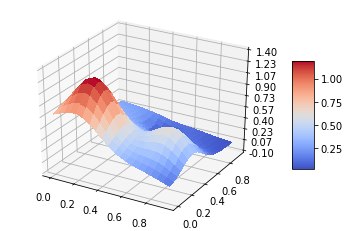
\includegraphics{franke_function}
    \caption{Franke function on $[0, 1]^2$}
    \label{fig:f1}
\end{figure}

\subsection{SRTM data}

SRTM stands for Shuttle Radar Topography Mission, ‘the best quality, freely available digital elevation models worldwide’ \cite{nik}. 

The dataset for this research contains the elevation data for a region close to Stavanger, Norway. The data basically is an 2d-array with length 3601 along the first axis and 1801 along the second axis with the corresponding height values stored inside it.

\begin{wrapfigure}{r}{0.25\textwidth}
    \centering
    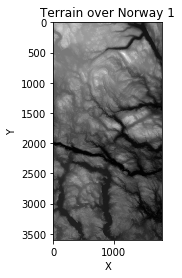
\includegraphics[width=0.25\textwidth]{terr_over_norway}
    \caption{Image of selected terrain data}
    \label{fig:f2}
\end{wrapfigure}

\subsection{General linear models}

The general linear model is written as:
\begin{equation*}
    \bm{y} = \bm{X} \bm{\beta} + \bm{\epsilon}
\end{equation*}
Where $\bm{y}$ is the set of data we are aiming to fit, $\bm{X}$ is the so-called design matrix, which exists of the input variables, $\bm{\beta}$ gives the regression parameters and $\bm{\epsilon}$ contains the errors; representing the noise in the data. 

\subsection{Ordinary Least Squares}

OLS (Ordinary Least Squares) is a method for estimating the unknown parameters in a linear regression model. By defining a function which gives the measure of the spread between the values $y_i$ (the values from the dataset) and $\tilde{y}_i$ (the predicted values), the optimal parameters $\beta_i$ can be found.  This gives the so-called cost function for $\bm{\beta}$:
\begin{equation*}
\begin{aligned}
    C(\bm{X}, \bm{\beta}) = \frac{1}{n} \sum_{i=0}^{n-1} (y_i - \tilde{y}_i)^2 &= \frac{1}{n} \Big\{(\bm{y} - \bm{\tilde{y}})^T(\bm{y} - \bm{\tilde{y}})\Big\} \\
    &= \frac{1}{n} \Big\{(\bm{y} - \bm{X}\bm{\beta})^T(\bm{y} - \bm{X}\bm{\beta})\Big\}
\end{aligned}
\end{equation*}
If the matrix $X^TX$ is invertible, the parameter $\bm{\beta}$ is defined as follows: 
\begin{equation*}
    \bm{\beta} = (\bm{X}^T\bm{X})^{-1} \bm{X}^T \bm{y}
\end{equation*}

\subsection{Ridge Regression}

When multicollinearity occurs in the design matrix (i.e. a (near-)singular design matrix), the variances of the OLS estimates are large, meaning they may be far from the true value. By adding a regularization parameter, Ridge regression reduces the standard errors. \cite{ncss}

The multicollinearity leads to that the matrix $X^TX$ is not invertible. By adding the regularization parameter $\lambda$ as diagonal component the matrix is invertible, i.e. $X^TX$ becomes $X^TX + \lambda I$, where $I$ is the identity matrix. The cost function for $\bm{\beta}$ then becomes:
\begin{equation*}
    C(\bm{X}, \bm{\beta}) = \frac{1}{n} \Big\{(\bm{y} - \bm{X}\bm{\beta})^T(\bm{y} - \bm{X}\bm{\beta})\Big\} + \lambda \bm{\beta}^T \bm{\beta}
\end{equation*}
And the estimate of $\bm{\beta}$ becomes: 
\begin{equation*}
    \bm{\beta} = (\bm{X}^T\bm{X} + \lambda \bm{I})^{-1} \bm{X}^T \bm{y}
\end{equation*}



\subsection{Lasso Regression}

Lasso offers another solution to multicollinearity in the design matrix. LASSO stands for Least Absolute Shrinkage and Selection Operator. It shrinks the data values towards a central point, by adding a regularization parameter $\lambda$, like in Ridge regression. The difference is that Lasso uses L1 regularization; instead of taking the square of the coefficients, magnitudes are taken into account. This can result in some coefficients becoming eliminated from the model, and therefore helps with feature selection as well. \cite{tds2} 

For lasso regression the cost function for $\bm{\beta}$ becomes: 

\begin{equation*}
    C(\bm{X}, \bm{\beta}) = \frac{1}{n} \Big\{(\bm{y} - \bm{X}\bm{\beta})^T(\bm{y} - \bm{X}\bm{\beta})\Big\} + \lambda \left \Vert \bm{\beta} \right \Vert_1
\end{equation*}

As $\lambda$ increases, more coefficients are set to zero and eliminated, and the more the bias increases. As $\lambda$ decreases, the variance increases. We elaborate more on bias and variance at the end of this section.  

\subsection{Resampling techniques}

Resampling techniques involve repeatedly drawing samples from a training set and refitting the model on each sample, to obtain additional information about the fitted model \cite{tds1}. There are several resampling methods, for this project specifically the k-fold cross-validation is used. In k-fold cross-validation the dataset is randomly divided into k subsets (i.e. the number of folds), each equally sized. The model is fitted on the k-1 training sets, and the remaining subset is used as test set. This is done multiple times, so that every subset is used as test data. In the end, the model is summarized by using the model evaluation scores for each sample\cite{lec}.

\subsection{Bias-variance tradeoff}

As we saw before, we find the parameters $\bm{\beta}$ via the cost-function: 

\begin{equation*}
    C(\bm{\tilde{y}}) = \frac{1}{n} \sum_{i=0}^{n-1} (y_i - \tilde{y}_i)^2
\end{equation*}

We can rewrite this as follows:

\begin{equation*}
\begin{aligned}
 &\mathds{E}[(\bm{y}-\bm{\tilde{y}})^2]\\
 &=\mathds{E}[(\bm{f}(\bm{x})+\bm{\epsilon}-\bm{\tilde{y}})^2]\\
 &= \mathds{E}[(\bm{f}(\bm{x})-\mathds{E}[\bm{\tilde{y}}]+\bm{\epsilon}-(\bm{\tilde{y}}-\mathds{E}[\bm{\tilde{y}}]))^2]\\
 &= \mathds{E}\Big[(\bm{f}(\bm{x})-\mathds{E}[\bm{\tilde{y}}])^2+\bm{\epsilon}^2+(\bm{\tilde{y}}-\mathds{E}[\bm{\tilde{y}}])^2+\bm{\epsilon}(\bm{f}(\bm{x})-\mathds{E}[\bm{\tilde{y}}])\\
 &\qquad \quad +\bm{\epsilon}(\mathds{E}[\bm{\tilde{y}}]-\bm{\tilde{y}})+(\bm{f}(\bm{x})-\mathds{E}[\bm{\tilde{y}}])(\mathds{E}[\bm{\tilde{y}}]-\bm{\tilde{y}})\Big]\\\
 &= \mathds{E}[(\bm{f}(\bm{x})-\mathds{E}[\bm{\tilde{y}}])^2] + \mathds{E}[\bm{\epsilon}^2] + \mathds{E}[(\bm{\tilde{y}}-\mathds{E}[\bm{\tilde{y}}])^2]\\
 &\quad+\mathds{E}[\bm{\epsilon}(\bm{f}(\bm{x})-\mathds{E}[\bm{\tilde{y}}])] +  \mathds{E}[\bm{\epsilon}(\mathds{E}[\bm{\tilde{y}}]-\bm{\tilde{y}})] + \mathds{E}\big[(\bm{f}(\bm{x})-\mathds{E}[\bm{\tilde{y}}])(\mathds{E}[\bm{\tilde{y}}]-\bm{\tilde{y}})\big]\\
 &= \mathds{E}[(\bm{f}(\bm{x})-\mathds{E}[\bm{\tilde{y}}])^2] + \mathds{E}[\bm{\epsilon}^2] + \mathds{E}[(\bm{\tilde{y}}-\mathds{E}[\bm{\tilde{y}}])^2]+ \mathds{E}[\bm{\epsilon}(\bm{f}(\bm{x})-\mathds{E}[\bm{\tilde{y}}])] \\
 &\quad+\mathds{E}[\bm{\epsilon}(\mathds{E}[\bm{\tilde{y}}]-\bm{\tilde{y}})] + (\bm{f}(\bm{x})-\mathds{E}[\bm{\tilde{y}}])\mathds{E}[\mathds{E}[\bm{\tilde{y}}]-\bm{\tilde{y}}]\\
  &= \mathds{E}[(\bm{f}(\bm{x})-\mathds{E}[\bm{\tilde{y}}])^2] + \mathds{E}[\bm{\epsilon}^2] + \mathds{E}[(\bm{\tilde{y}}-\mathds{E}[\bm{\tilde{y}}])^2]+ (\bm{f}(\bm{x})-\mathds{E}[\bm{\tilde{y}}])\mathds{E}[\bm{\epsilon}] \\
 &\quad+(\mathds{E}[\bm{\tilde{y}}]-\bm{\tilde{y}})\mathds{E}[\bm{\epsilon}] + (\bm{f}(\bm{x})-\mathds{E}[\bm{\tilde{y}}])(\mathds{E}[\bm{\tilde{y}}]-\mathds{E}[\bm{\tilde{y}}])\\
&= \mathds{E}[(\bm{f}(\bm{x})-\mathds{E}[\bm{\tilde{y}}])^2] + \mathds{E}[(\bm{\tilde{y}}-\mathds{E}[\bm{\tilde{y}}])^2] + \mathds{E}[\bm{\epsilon}^2]\\
 &= \frac{1}{n} \sum_{i=1}^n (f_i - \mathds{E}[\bm{\tilde{y}}])^2 + \frac{1}{n} \sum_{i=1}^n (\tilde{y}_i - \mathds{E}[\bm{\tilde{y}}])^2 + \sigma^2
\end{aligned}
\end{equation*}

In this formula, the left side gives the total error, and the first part of the right side is the bias squared, the second part is the variance and the last part the variance of the error, or the irreducible error in the data \cite{elemstat}.

The bias is the difference between the average prediction of the model and the correct value which we are trying to predict. Models with a high bias oversimplify the model which leads to underfitting. Variance is the variability of model prediction for a given data point. Models with a high variance do not generalize and have high error rates on unseen (test) data; i.e. overfitting \cite{elemstat}. The bias-variance tradeoff deals with finding the right balance between this bias and variance, which minimizes the total error.


\subsection{Model evaluation}

The regression models are evaluated using two different criteria: the MSE (Mean Squared Error) and the $R^2$ score. 
The MSE is a measure of the quality of an estimator, and the smaller the value the better the fit (where zero is a perfect fit). The MSE is calculated by: 
\begin{equation*}
  \textrm{MSE}(\bm{x}, \bm{y}) = \frac{1}{n} \sum_{i=1}^n (x_i - y_i)^2
\end{equation*}
The $R^2$ score is the coefficient of determination, it indicates how well observed outcomes are replicated by the model. The best possible score is 1.0, whereas a negative $R^2$ score indicates that the model performs worse than just taking the mean. The $R^2$ score is given by:
\begin{equation*}
\begin{aligned}
   R^2(\bm{y}, \bm{\tilde{y}}) = 1 - \frac{\sum_i (y_i - \tilde{y}_i)^2}{\sum_i (y_i - \bar{y})^2} \quad \textrm{,where} \quad \bar{y} = \frac{1}{n} \sum_{i=1}^n y_i
\end{aligned}
\end{equation*}

\section{Code implementation}

In this section we will explain some parts of our code implementation. The jupyter notebook with the code for the Franke function (‘Regression methods Franke Function) and for the terrain data (‘Regression methods Terrain Data’) can be found at the following link: 

\begin{center}
    \href{https://github.com/jolyndev/FYS-STK4155}{\textbf{Github repository}}
\end{center}

\subsection{Regression methods for the Franke function}

For the Franke function the design matrix is set up as follows: 

\begin{lstlisting}
def CreateDesignMatrix_X(x, y, n):
    if len(x.shape) > 1:
        x = np.ravel(x)
        y = np.ravel(y)
        
    N = len(x)
    l = int((n+1)*(n+2)/2)
    X = np.ones((N,l))
        
    for i in range(1,n+1):
        q = int((i)*(i+1)/2)
        for k in range(i+1):
            X[:,q+k] = x**(i-k) * y**k
    return X
\end{lstlisting}

Where x and y are given by a number of points between 0 and 1, and n is the degree of the polynomial.
The true function is the Franke function without the added noise. Normally not available, but since we have it we might as well use it.

The MSE and R2-score are given by the following functions:

\begin{lstlisting}
def MSE(z_data, z_model):
    n = np.size(z_model)
    return np.sum((z_data-z_model)**2)/n
print(MSE(z_true, ztilde))

def R2(z_data, z_model):
    return 1 - np.sum((z_data - z_model) ** 2) / np.sum((z_data - np.mean(z_model)) ** 2)
print(R2(z_true, ztilde))

\end{lstlisting}

The cross-validation is implemented with the following function:

\begin{lstlisting}
def cross_validation(x, y, k):
    n = len(x)
    indexes = np.arange(y.shape[0])
    np.random.shuffle(indexes)
    x = x[indexes]
    y = y[indexes]
    r2_test = []
    mse_test = []
    for i in range(k):
        x_train = np.concatenate((x[:int(i*n/k)], x[int((i + 1)*n/k): ]), axis = 0)
        x_test = x[int(i*n/k):int((i + 1)*n/k)]
        y_train = np.concatenate((y[:int(i*n/k)], y[int((i + 1)*n/k): ]), axis = 0)
        y_test = y[int(i*n/k):int((i + 1)*n/k)]
        beta = np.linalg.inv(x_train.T.dot(x_train)).dot(x_train.T).dot(y_train)
        ytilde = x_train @ beta
        ypredict = x_test @ beta
        mse_test.append(MSE(y_test, ypredict))
        r2_test.append(R2(y_test, ypredict))
    r2_test = np.array(r2_test)
    mse_test = np.array(mse_test)
    return r2_test, mse_test

\end{lstlisting}

Where k is the number of folds. This function returns everything we need to cross-validate. The same cross-validation function is used for Ridge regression, where beta is replaced with the definition that gives the beta for Ridge. 
Ridge regression is implemented as follows:

\begin{lstlisting}
X = X_train
Y = X_test
b_r = np.linalg.inv(X.T.dot(X)+(lmb*np.eye(len(X[0])))).dot(X.T).dot(z_1)
zridge = X @ b_r
ridge_predict = Y @ b_r
\end{lstlisting}

With the following code for GridSearchCV of sklearn to find the optimal value for lambda. 

\begin{lstlisting}
ridge = skl.Ridge()
ridge_regressor = GridSearchCV(ridge, param_grid, scoring='neg_mean_squared_error', cv=kfold)
ridge_regressor.fit(X_new[:,1:], z_1)
print(ridge_regressor.best_params_)
print(ridge_regressor.best_score_)
nlambdas = 50
lambdas = np.logspace(-7, 2, nlambdas)
param_grid = {'alpha': lambdas}
\end{lstlisting}

The LASSO regression is implemented as follows: 

\begin{lstlisting}
clf_lasso = skl.Lasso(alpha=l_lambda, precompute = True, tol = 10, max_iter = 10e3).fit(X_new_train, z_new_train)
pred_lasso = clf_lasso.predict(X_new_test)
\end{lstlisting}

To validate our own algorithms they are compared with the corresponding sk-learn functionalities. To verify the results sometimes an easier plot is used (for example one without cross-validation and one with cross-validation, to make sure it is comparable.

\subsection{Regression methods for the terrain data}

For the terrain data we basically used the same functions, with a few tweaks. To start, the terrain data has been standardised, because the values are very big. This has been done by subtracting the mean and dividing by the standard deviation. Since we have a lot of data, we wanted to make our array smaller to make computations easier. Therefore, we remove the last column and row to get a 3600 by 1800 array which we now can make smaller by setting the new value as the average over a small array inside our 3600 by 1800 array, to get an 400 by 200 array. For these purposes, we used this code.

\begin{lstlisting}
def rebin(a, shape):
    sh = shape[0],a.shape[0]//shape[0],shape[1],a.shape[1]//shape[1]
    return a.reshape(sh).mean(-1).mean(1)
    
terrain1 = terrain1[:3600, :1800]
terrain1 = (terrain1 - np.mean(terrain1)*np.eye(terrain1.shape)) / np.std(terrain1)
terrain1 = rebin(terrain1, (3600//9, 1800//9))
\end{lstlisting}

% The vectors x and y each have a length of 250, which results in $250^2$ datapoints.

\section{Results and discussion}

This section starts with presenting the results of the three regression methods on the Franke function, and a discussion of these results. The section continues with the results of the regression mehtods on the SRTM data, and ends with a discussion of which regression method fits the SRTM data the best.

\subsection{OLS regression}

After creating the data with 250 data points in x and y and a polynomial degree of 5, we start with fitting an OLS regression model to the data. The data is split into 80\% training data and 20\% test data.

% \begin{figure}
%     \centering
%     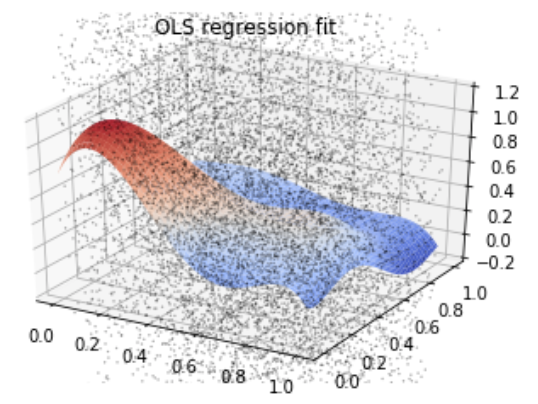
\includegraphics{1}
%     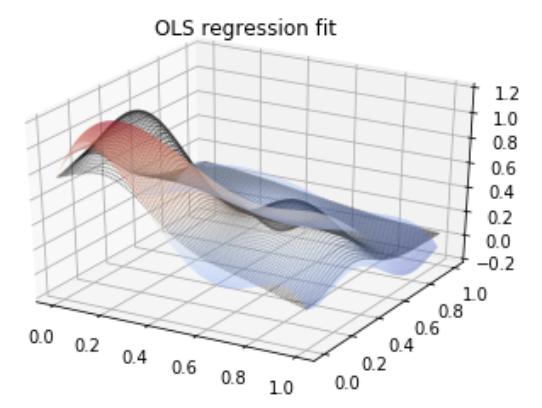
\includegraphics{2}
%     \caption{}
%     \label{fig:f3}
% \end{figure}

\begin{figure}
    \centering
    \begin{subfigure}{.5\textwidth}
        \centering
        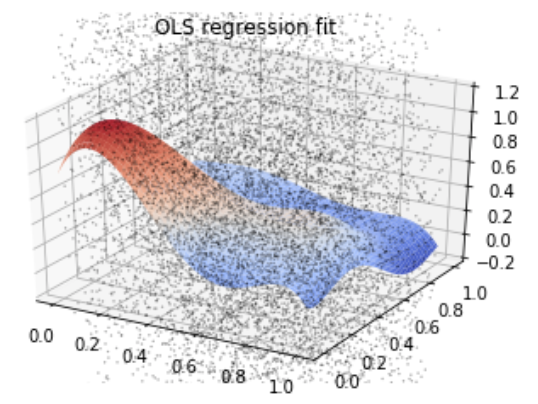
\includegraphics[width=.85\linewidth]{1}
        \caption{OLS regression fit with the noisy data}
        \label{fig:f3sub1}
    \end{subfigure}%
    \begin{subfigure}{.5\textwidth}
        \centering
        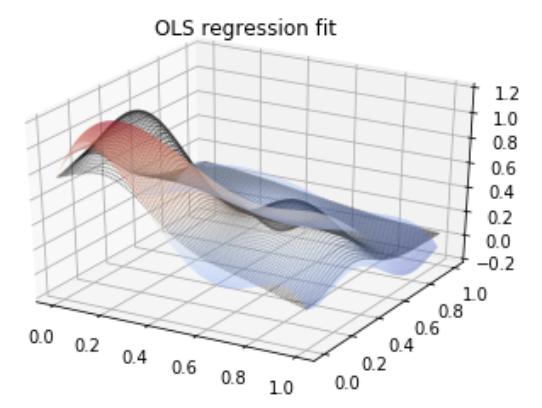
\includegraphics[width=.85\linewidth]{2}
        \caption{OLS regression fit with the real data}
        \label{fig:f3sub2}
    \end{subfigure}
    % \caption{OLS regression}
    \label{fig:f3}
\end{figure}

% \begin{figure}%
%     \centering
%     \subfloat[label 1]{{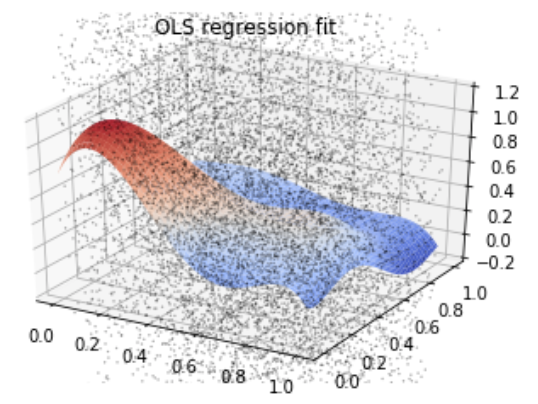
\includegraphics[width=5cm]{1} }}%
%     \qquad
%     \subfloat[label 2]{{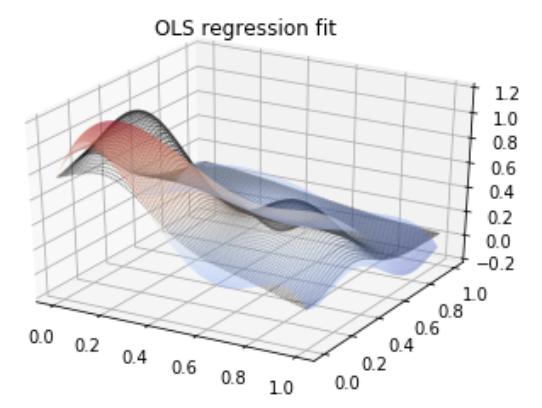
\includegraphics[width=5cm]{2} }}%
%     \caption{2 Figures side by side}%
%     \label{fig:example}%
% \end{figure}

Figure \ref{fig:f3sub1} shows the noisy data (Franke function with added noise), and a colored surface plot of the fitted OLS regression on this (noisy) data. Figure \ref{fig:f3sub2} shows the scattered data (the black dots) of the real data (the Franke function without the noise), and a colored surface plot of the same fit of the OLS regression (on the noisy data). All the models are always trained on the noisy data, where the goal is to predict the real function as good as possible.

Next we can compute the MSE-score and $R^2$-score for the training, test and the real data.

\begin{table}
  \begin{center}
    \caption{MSE- and $R^2$-scores for OLS regression with polynomial degree 5.}
    \label{tab:table1}
    \begin{tabular}{l|c|c} 
      \textbf{ } & \textbf{MSE-score} & \textbf{R2-score}\\
      \hline
      Training data & 1.010 & 0.071\\
      Test data & 1.020 & 0.077\\
      Real function data & 0.002 & 0.971\\
    \end{tabular}
  \end{center}
\end{table}


We observe a big difference between the MSE-score for the training and test data and the MSE-score for the true data. This is due to the noise we’ve added to the Franke function. The noise is added with a multiplication of 1, which is why the MSE-score is around 1. The $R^2$-score also differs greatly for the training and test data and the true data. However, seeing that we want the model to predict the ‘real’ data (i.e. the true function), the $R^2$-score for the real function is most relevant one. The MSE- and $R^2$-score for the real data are both very good, showing that the OLS regression model with polynomial degree 5 is a pretty good fit. We also have a quick look at the confidence interval \footnote{\textit{Important footnote: The calculation and result of the confindence intervals (actually more so of the variance) is wrong and doesn't make sense. Currently we are not taking the variance out of the diagonal elements of $(X^T X)^{-1}$. Unfortunately, there is no time left to fix this pretty big mistake :(}} of the coefficients. The 95\% confidence intervals are calculated as follows, using a Z-score of 1.96, where $\mu$ is the mean of $\bm{\beta}$, $\sigma$ is the standard deviation of $\bm{\beta}$, and $n$ is the length of $\bm{\beta}$:  
\begin{equation*}
    \left(\mu - 1.96 \frac{\sigma}{\sqrt{n}}, \mu + 1.96 \frac{\sigma}{\sqrt{n}}\right)
\end{equation*}
Which gives the following values:

\begin{table}
  \begin{center}
    \caption{Confidence intervals for $\bm{\beta}$ (OLS, polynomial degree = 5).}
    \label{tab:table2}
    \begin{tabular}{l|c|c} 
      \textbf{Mean} & \textbf{CI-interval low} & \textbf{CI-interval high}\\
      \hline
      0.004 & -54.018 & 12.305\\
    \end{tabular}
  \end{center}
\end{table}


The confidence interval tells us how sure we are that the true mean is in the interval, in this case 95\% sure that it is between -12.302 and 12.305.

In the next sections we will see if we can optimize our OLS fit further, by trying to minimize the MSE-score.


\subsubsection{K-fold cross-validation}

Instead of using a train-test split, which tests our data on a small test set (20\% of the dataset), we will use cross-validation to assess the model. We use a k of 10, meaning that we do a 10-fold cross-validation, where the data is split into 10 parts (i.e. folds, randomly picked), the model is trained on 9 parts (90\% of the data) and is tested on the remaining part (10\% of the data), which is done 10 times. That means that all the data has been used as both training and once as test data.

\begin{table}
  \begin{center}
    \caption{MSE- and $R^2$-scores for cross-validated OLS regression with polynomial degree 5.}
    \label{tab:table3}
    \begin{tabular}{l|c|c|c|c} 
      & \textbf{MSE-score} & \textbf{MSE-score} & \textbf{R2-score} & \textbf{R2-score}\\
      & & \textbf{CV (std)} & & \textbf{CV (std)}\\
      \hline
      Training data & 1.010 & 1.012 (+/- 0.003) & 0.071 & 0.072 (+/- 0.002)\\
      Test data & 1.020 & 1.013 (+/- 0.025) & 0.077 & 0.071 (+/- 0.010)\\
      Real function data & 0.002 & N/A & 0.971 & N/A\\
    \end{tabular}
  \end{center}
\end{table}


The MSE- and $R^2$-scores for the 10 CV-folds are averaged and displayed in table \ref{tab:table1}, together with the standard deviation of these 10 scores. We see that the standard deviations are fairly low, which means that the model has a consistent performance on different test sets. We also see that the scores for OLS without cross-validation fall in the range of the CV-scores and their standard deviation. 

The MSE- and $R^2$-score for the real data is not available anymore unfortunately, because otherwise we would have to test the model on the real data as well. We will optimize the MSE-score for the test data.

The SVD and pseudo-inverse
A standard matrix inversion might lead to (near-) singular matrices. To prevent this, we can use the SVD (Singular Value Decomposition). However, we found out fairly late that the reason that our MSE-score exploded after the 13th/14th polynomial degree was probably due to this singularity (the higher the polynomial degree, and the bigger the design matrix, the bigger the chance on near-singularity). Seeing that we did not have a lot of time left, we decided not to implement the SVD-algorithm from scratch, but we used Numpy’s pinv, which computes the pseudo-inverse of a matrix, using its singular value decomposition (tip given at the data lab).

\subsubsection{Complexity of the model}

Using our code for cross-validation, we will start to optimize our OLS regression model. We start by looking at which polynomial degree (i.e. the complexity of the model) fits the data the best.

\begin{figure}
    \centering
    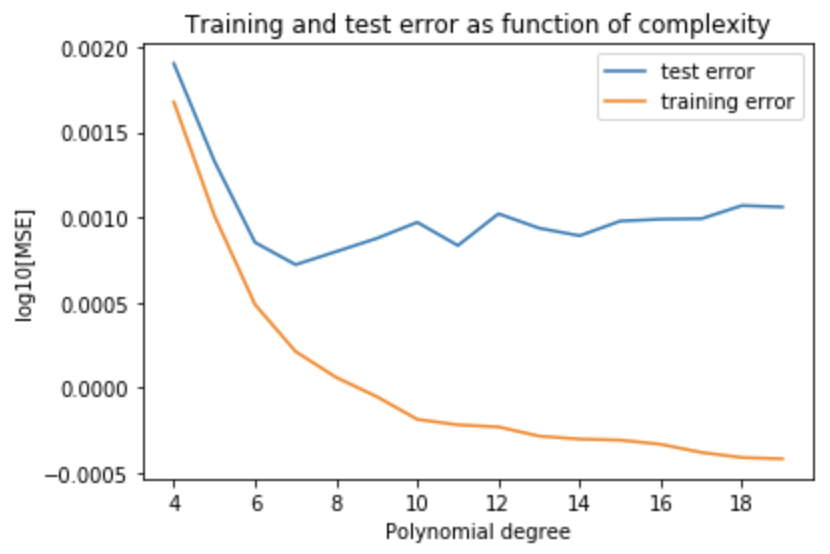
\includegraphics{3}
    \caption{Training and test error as a function of complexity}
    \label{fig:f4}
\end{figure}

The lines are plotted starting at a polynomial degree of 4 (appendix 1 shows the graph from degree 1, which is harder to interpret). The graph shows that the training error will decrease when the complexity increases, this is because the model will start to fit every point in the training data. However, if we would let the model do this, it would not be able anymore to perform on unseen data, because it has fitted all the noise in the training data as well. This is called overfitting. We can see that our model performs best for a polynomial degree of 7, because from this point the test error starts rising again. In appendix 1 is also a plot for the error on the true data, which confirms this.

\subsubsection{Bias-variance trade-off}

Now we can plot the bias and the variance for the OLS regression model.

\begin{figure}
    \centering
    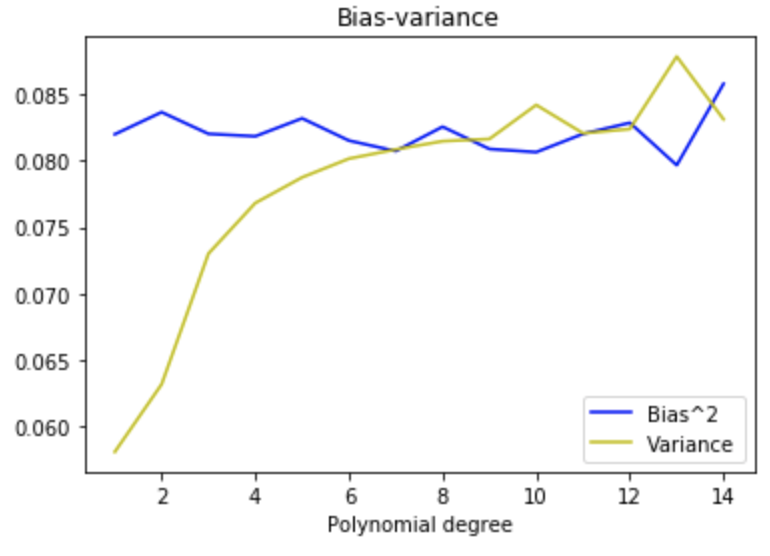
\includegraphics{4}
    \caption{Bias and variance plotted against complexity}
    \label{fig:f5}
\end{figure}

We see that for a polynomial of 7, there is a good tradeoff between the bias and the variance. It is where they first cross, and where the variance is not that high yet and the bias is not too low. However, we can also see that for our data, the bias-variance tradeoff looks a bit different. The variance shows a logarithmic growth instead of an exponential growth. This could happen if the different data points in the data are far from each other. If we look at the Franke function, we see that it has a relatively high peak and a few dips, meaning that when the complexity of the model increases it will go towards these peaks and dips, which will cause the variance to rise quickly.

The bias for the model seems to be decreasing, however very gentle. This could be due to the amount of noise in the model, and to the number of data points. The added noise is normal distributed, meaning it is everywhere. So when the model is not complex, it does not capture the function points, which cause the bias. But when the model gets more complex, it captures the function better, but not the noise in the middle anymore. Because we have a lot of data points, the model is not overfitting yet at a polynomial degree of 15. Eventually, when the complexity goes towards infinity, the bias will decrease because the model will capture both the data points and the noise.

Now we can compare the results for the OLS regression model for a polynomial degree of 5 and a polynomial degree of 7.

\begin{table}
  \begin{center}
    \caption{MSE- and $R^2$-scores for OLS regression with polynomial degree 5 and polynomial degree 7.}
    \label{tab:table4}
    \begin{tabular}{l|c|c} 
      \textbf{ } & \textbf{Polynomial degree = 5} & \textbf{Polynomial degree = 7}\\
      \hline
      MSE-score & 1.013 (+/- 0.020) & 1.012 (+/- 0.023)\\
      R2-score & 0.071 (+/- 0.020) & 0.072 (+/- 0.010)\\
      MSE real function & 0.0024 & 0.0014\\
    R2 real function & 0.971 & 0.983\\
    \end{tabular}
  \end{center}
\end{table}


We see that for a polynomial degree of 7 all the scores are better.

We also compare the 95\% confidence intervals of the 5th order polynomial and the 7th order polynomial.

\begin{table}
  \begin{center}
    \caption{Confidence intervals for $\bm{\beta}_{\text{OLS}}$.}
    \label{tab:table5}
    \begin{tabular}{l|c|c|c} 
      & \textbf{Mean} & \textbf{CI-interval low} & \textbf{CI-interval high}\\
      \hline
    OLS, polynomial degree 5 & 0.004 & -54.018 & 54.026\\
    OLS, polynomial degree 7 & -0.004 & -821.563 & 821.556\\
    \end{tabular}
  \end{center}
\end{table}


We see that the interval has become much larger, while the mean is still around zero. This difference is explained by the fact that the polynomial degree has increased, which means that the standard deviation of the coefficients are further apart, and the confidence interval increases.

Now we will have a look at Ridge and LASSO regression to see if these methods can optimize our fit more.

\subsection{Ridge regression}

For Ridge we need to find the optimal value of the hyperparameter $\lambda$. We can find this value by plotting the MSE-score and the value of $\lambda$.

\begin{figure}
    \centering
    \begin{subfigure}{.5\textwidth}
        \centering
        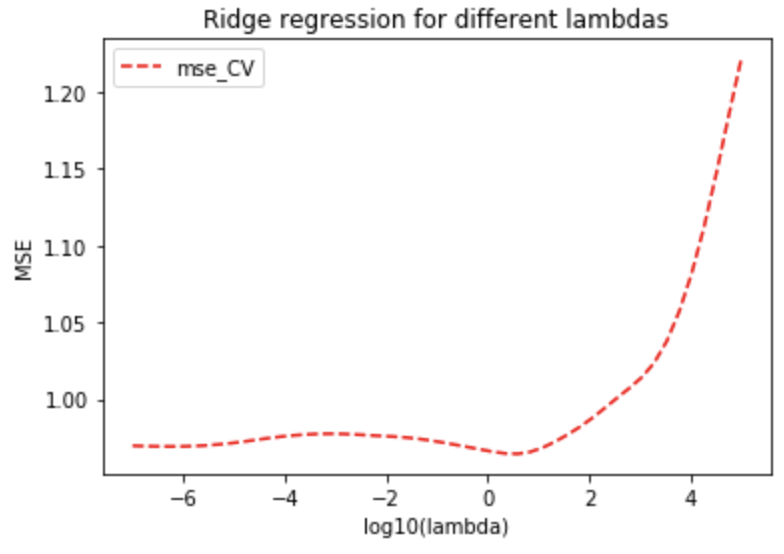
\includegraphics[width=.9\linewidth]{5}
        \caption{OLS regression with the noisy data}
        \label{fig:f6sub1}
    \end{subfigure}%
    \begin{subfigure}{.5\textwidth}
        \centering
        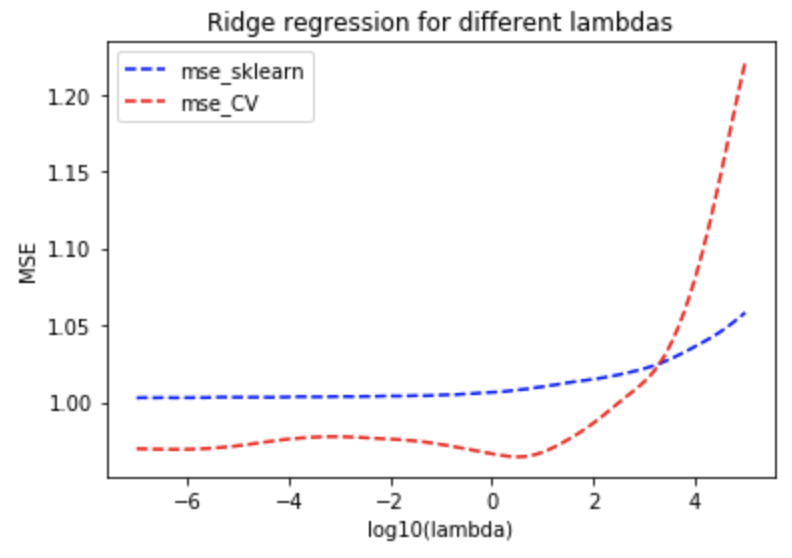
\includegraphics[width=.9\linewidth]{6}
        \caption{OLS regression with the real data}
        \label{fig:f6sub2}
    \end{subfigure}
    \caption{Graphs showing correlation between $\lambda$ and MSE-score}
    \label{fig:f6}
\end{figure}

However, as seen in figure \ref{fig:f6sub1}, we see a small dip in the MSE-score for a $\lambda$ of 1. However, if we compare the graph with the build-in Ridge regression of SciKit learn (figure \ref{fig:f6sub2}) and when we look at the dependence on $\lambda$ for different polynomial degrees (figure \ref{fig:f7sub2}), we see that a $\lambda$ of 1 does not give the best score. Meaning that our own code for the plot does not show the actual values.

\begin{figure}
    \centering
    \begin{subfigure}{.5\textwidth}
        \centering
        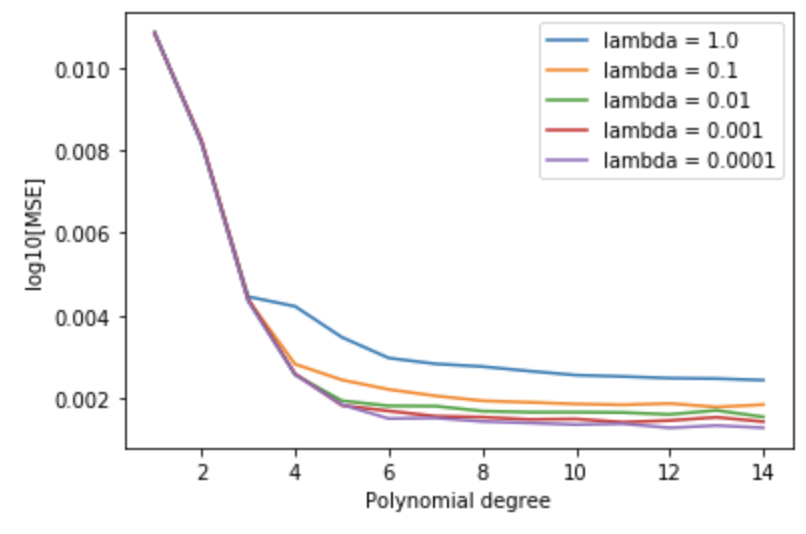
\includegraphics[width=.9\linewidth]{7}
        \caption{Model complexity and lambda}
        \label{fig:f7sub1}
    \end{subfigure}%
    \begin{subfigure}{.5\textwidth}
        \centering
        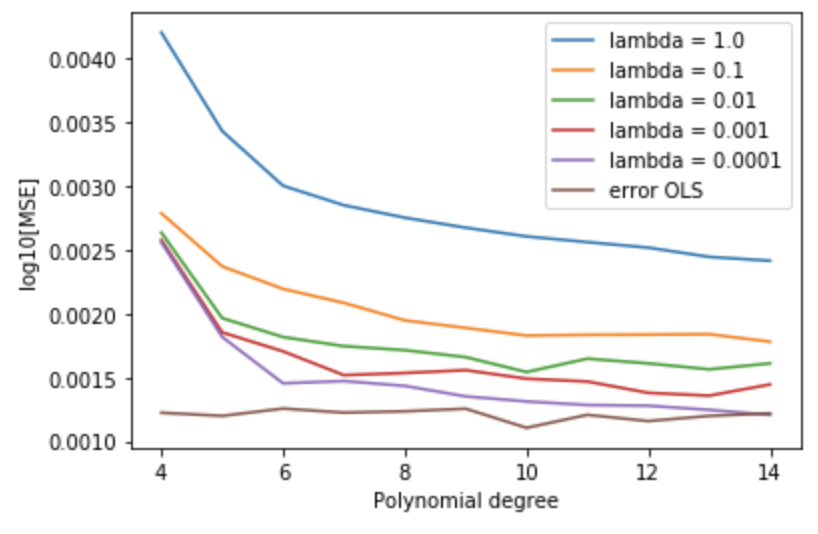
\includegraphics[width=.9\linewidth]{8}
        \caption{Complexity and lambda with OLS}
        \label{fig:f7sub2}
    \end{subfigure}
    \caption{Relation between complexity, $\lambda$ and MSE-score}
    \label{fig:f7}
\end{figure}

We see that the Ridge-regression MSE-scores steadily go down, and that some (the lower $\lambda$ values) seem to flatten out after the 14th degree. When we compare this to the MSE of the OLS regression (figure \ref{fig:f8}), we see that the MSE-score for the OLS regression is still lower than the MSE-scores for Ridge regression. Moreover, e see that when $\lambda$ increases, the MSE-score increases as well. The closer $\lambda$ gets to zero, the smaller the MSE-score. When $\lambda$ would have a value of zero, the diagonal that is added to the matrix is zeroed out, which means we are performing a regular OLS. 
\subsubsection{Bias-variance trade-off Ridge}

Looking at the bias-variance tradeoff for Ridge for different $\lambda$'s we observe the following graph.

\begin{figure}
    \centering
    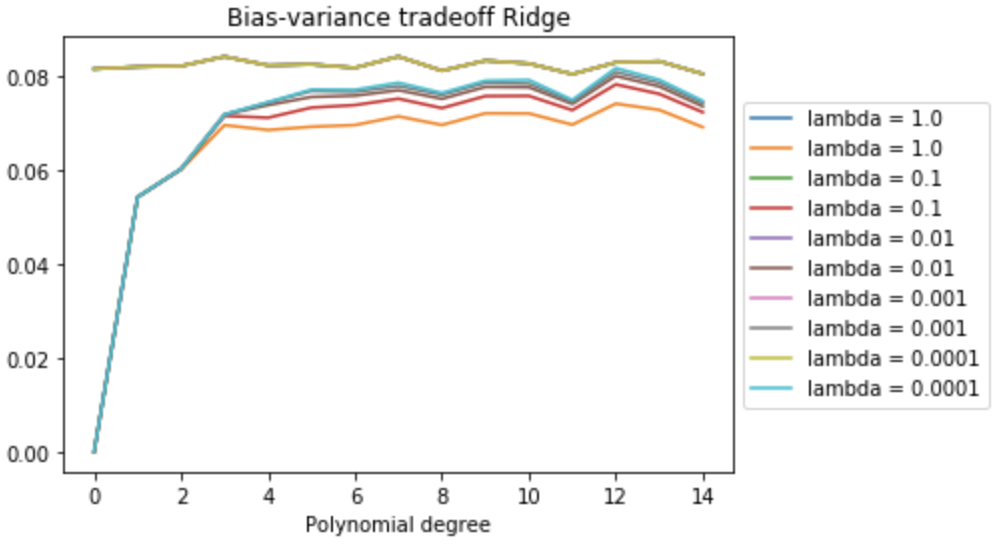
\includegraphics[width=.8\linewidth]{9}
    \caption{Error plotted against complexity}
    \label{fig:f8}
\end{figure}

\begin{figure}
    \centering
    \begin{subfigure}{.5\textwidth}
        \centering
        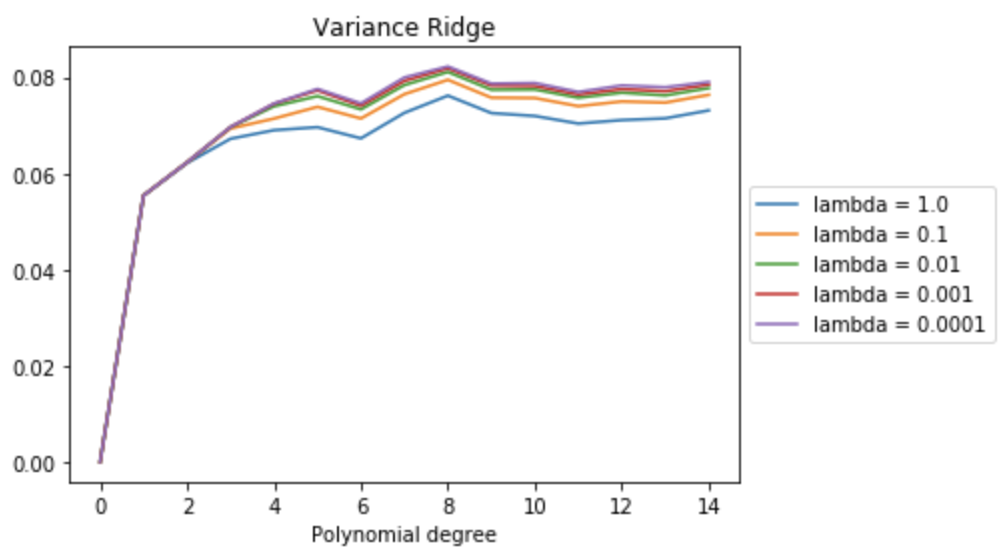
\includegraphics[width=.95\linewidth]{10}
        % \caption{OLS regression fit with the noisy data}
        \label{fig:f9sub1}
    \end{subfigure}%
    \begin{subfigure}{.5\textwidth}
        \centering
        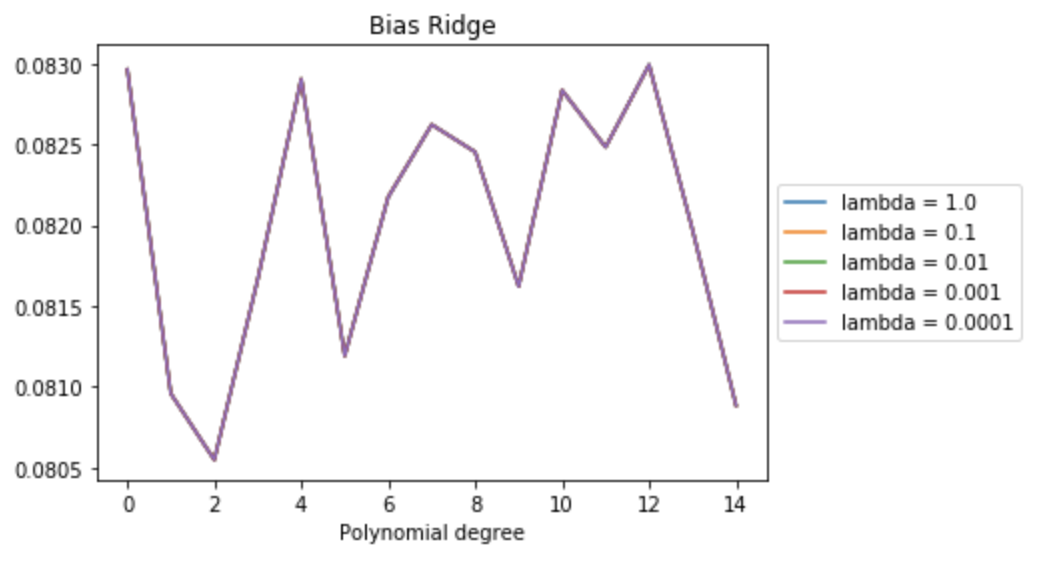
\includegraphics[width=.95\linewidth]{11}
        % \caption{OLS regression fit with the real data}
        \label{fig:f9sub2}
    \end{subfigure}
    \caption{Variance and Bias depending on model complexity and $\lambda$}
    \label{fig:f9}
\end{figure}

Ridge regression shrinks the coefficients towards zero, so it decreases the variance of beta, so when $\lambda$ increases the variance decreases. If we look at figure \ref{fig:f7sub2}, we see that for $\lambda$ = 1.0 the variance is the lowest. Furthermore, the graph of the variance is comparable to the variance graph for OLS.  The bias, on the other hand, should increase when a greater value for $\lambda$ is used. Because the coefficients are shrunk more towards zero for a greater value of $\lambda$, the estimated values will be further away from the actual values. Figure \ref{fig:f7sub2} is a plot of the bias for different values of $\lambda$, however the graph does not explain this theory, seeing that the bias does not change for different values of $\lambda$ here. Using graph Xa, we see the same result as for OLS regression, the bias seems to decrease very slowly.

For the confidence intervals we observe the following:

\begin{table}
  \begin{center}
    \caption{Confidence intervals for coefficients of $\bm{\beta}$.}
    \label{tab:table6}
    \begin{tabular}{l|c|c|c} 
      & \textbf{Mean} & \textbf{CI-interval low} & \textbf{CI-interval high}\\
      \hline
    OLS, polynomial degree 5 & 0.004 & -54.018 & 54.026\\
    OLS, polynomial degree 7 & -0.004 & -821.563 & 821.556\\
    Ridge regression & -0.003 & -807.303 & 807.296\\
    \end{tabular}
  \end{center}
\end{table}


The confidence intervals for ridge are lower, which makes sense, because Ridge shrinks the coefficient towards zero. Because we use a very small value for $\lambda$, the difference is not that big.

\subsection{Lasso regression}

For the LASSO regression we use the build-in functionality of SciKit-learn. We can make the same plot for $\lambda$ as we did for the Ridge regression. The graph for LASSO also shows that for a bigger value of $\lambda$ the error will increase, indicating that LASSO is not a better method than OLS for this dataset.

\begin{figure}
    \centering
    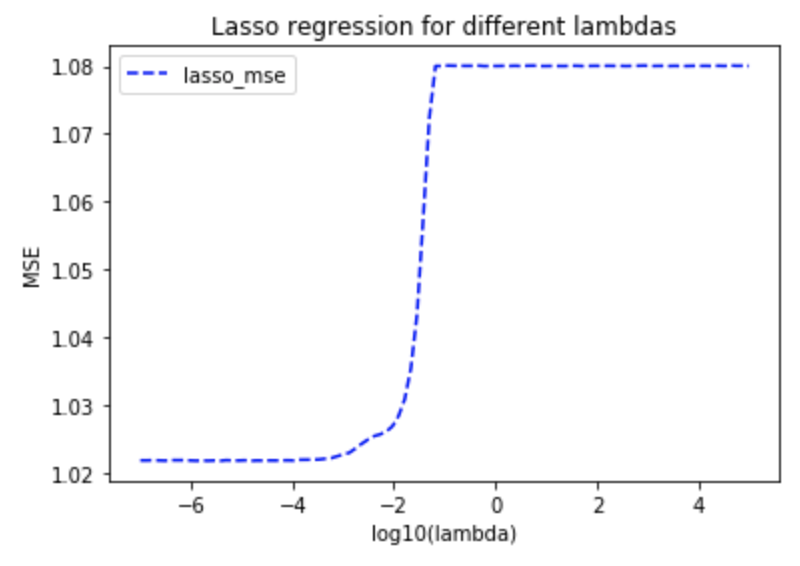
\includegraphics[width=0.9\linewidth]{12}
    \caption{In search of the best $\lambda$}
    \label{fig:f10}
\end{figure}

For LASSO, when $\lambda$ increases, the bias increases as well. When $\lambda$ decreases, the variance increases. For the confidence intervals we observe the following:

\begin{table}
  \begin{center}
    \caption{Confidence intervals for coefficients of $\bm{\beta}$.}
    \label{tab:table7}
    \begin{tabular}{l|c|c|c} 
      \textbf{ } & \textbf{Mean} & \textbf{CI-interval low} & \textbf{CI-interval high}\\
      \hline
    OLS, polynomial degree 5 & 0.004 & -54.018 & 54.026\\
    OLS, polynomial degree 7 & -0.004 & -821.563 & 821.556\\
    Ridge regression & -0.003 & -807.303 & 807.296\\
    Lasso regression & -0.029 & -0.318 & 0.261
    \end{tabular}
  \end{center}
\end{table}


We see that the confidence intervals for LASSO are very small. This could be due to the fact that LASSO shrinks and eliminates coefficients, which results in a low standard deviation between the coefficients.

\subsubsection{Comparison of models}

Finally we can compare the scores of the different models. To find the final optimal values of $\lambda$ for Ridge and LASSO we use SciKit-learn’s GridSearchCV, which uses a cross-validated grid search to find the lowest MSE-score for a certain value of $\lambda$. Using this, the optimal values for $\lambda$ for both Ridge and LASSO are $10^{7}$. The values of $\lambda$ to search between were from $10^{7}$ to $10^{2}$, given that GridSearchCV gives the lowest value here indicates that it would go further to zero, towards OLS regression, if possible. However, we can compare the results:

\begin{table}
  \begin{center}
    \caption{Regression results, K-fold CV with k=10.}
    \label{tab:table8}
    \begin{tabular}{l|c|c|c} 
      & \textbf{OLS} & \textbf{Ridge} ($\lambda = 10^{-7}$) & \textbf{LASSO} ($\lambda = 10^{-7}$)\\
      \hline
      MSE-score & 1.012 (+/- 0.023) & 1.012 (+/- 0.044) & 1.027 (+/- 0.032)\\
    R2-score & 0.072 (+/- 0.010) & 0.072 (=/- 0.010) & 0.058 (+/- 0.008)\\
    \end{tabular}
  \end{center}
\end{table}


We see that OLS and Ridge perform almost equally, while the LASSO regression is notably worse.

The reason for LASSO regression to perform bad on this dataset could be explained by that apparently the features in the dataset are not correlated. Since LASSO applies an ‘automatic feature selection’ by reducing some coefficients to zero, some variables could be eliminated. It also regulates the parameters. So it eliminates and shrinks features at the same time. Because our dataset is quite large, the risk of overfitting is fairly low. When applying LASSO, the model is most likely underfitting the data, due to the elimination and shrinkage of the coefficients. For LASSO the same applies as with Ridge, when $\lambda$ is zero we have a regular OLS regression.  

The scores for OLS and Ridge are almost the same, however, the standard deviation scores are slightly lower for OLS. Because $\lambda$ is very small, and Ridge does not set coefficients to zero, but shrinks them towards zero, the results are almost the same as for OLS. The reason why Ridge is not better than OLS could be; for a large value of $\lambda$ the variance decreases but the bias increases. Since we have a lot of data, the model won’t overfit quickly. So when applying Ridge, $\lambda$ goes almost to zero for the lowest error, seeing that otherwise the bias of the model will increase. We saw in the graph of the bias-variance tradeoff for OLS (figure \ref{fig:f8}) that the bias is very low for this model, so when applying Ridge the bias will be greater for every value of $\lambda$ then it is for OLS, explaining that OLS is a better fit for this data. 

Lastly, we can compare the scores for the real data for the three models. Here we see the same results, OLS and Ridge are almost the same (the difference is further down in the scores), while LASSO is arbitrarily worse.

\begin{table}
  \begin{center}
    \caption{Regression results on the real function.}
    \label{tab:table9}
    \begin{tabular}{l|c|c|c} 
      & \textbf{OLS} & \textbf{Ridge} ($\lambda = 10^{-7}$) & \textbf{LASSO} ($\lambda = 10^{-7}$)\\
      \hline
      Real function: MSE-score & 0.001 & 0.001 & 0.019\\
      Real function: $R^2$-score & 0.983 & 0.983 & 0.765\\
    \end{tabular}
  \end{center}
\end{table}


\subsection{SRTM data}

\begin{figure}
    \centering
    \begin{subfigure}{.5\textwidth}
        \centering
        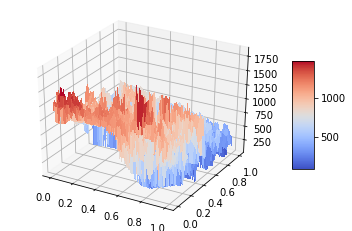
\includegraphics[width=.95\linewidth]{t1}
        \caption{Terrain data}
        \label{fig:t1sub1}
    \end{subfigure}%
    \begin{subfigure}{.5\textwidth}
        \centering
        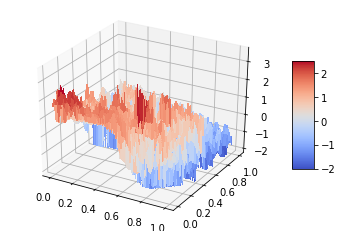
\includegraphics[width=.95\linewidth]{t2}
        \caption{Terrain data downsampled}
        \label{fig:t1sub2}
    \end{subfigure}
    \caption{The real data!}
    \label{fig:t1}
\end{figure}

Firstly, we normalize the terrain data and use a grid with values between 0 and 1. The original data can be seen in figure \ref{fig:t1sub1}, where as the data after downsampling from an 3600 by 1800 to 400 by 200 array can be seen in figure \ref{fig:t1sub2} and it seems like we are not losing to much information yet. And just for a nice picture, we are creating an model without any test data which you can see in figure \ref{fig:t2}.

\begin{figure}
    \centering
    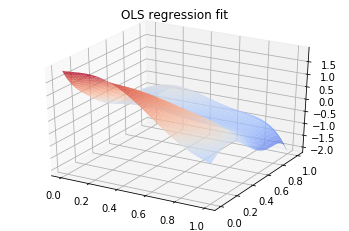
\includegraphics{t4}
    \caption{Fit for a nice picture}
    \label{fig:t2}
\end{figure}

\subsubsection{OLS regression}

Using 80 percent of the data as training data and 20 percent as test data and applying the OLS algorithm, we get MSE scores of roughly 0.46 for a design matrix which is based on polynomials up to fifth order. And the $R^2$ score is 0.538, which actually doesn't seem that bad and is better than the score for the Franke function. This is probably due to not a lot of error being in the terrain data since measuring the height with modern technology probably doesn't have a big error.

When using 10-fold cross-validation, very similar values compared to without the cross-validation for the MSE and $R^2$ score appear, when taking the mean, as you can see in \ref{tab:t1}. The standard deviation for MSE is between 0.0157 and the standard deviation $R^2$ score is 0.011.

\begin{table}
  \begin{center}
    \caption{MSE and $R^2$ for OLS on real data for degree 5}
    \label{tab:t1}
    \begin{tabular}{l|c|c} 
      & \textbf{MSE Test} & \textbf{$R^2$ Test}\\
      \hline
      OLS & 0.455 & 0.549\\
      10-fold CV & 0.458(+/- 0.16) & 0.540(+/- 0.012)\\
    \end{tabular}
  \end{center}
\end{table}

When we change the degree of the polynomials on which the design matrix is based on, we see from degree 1 to degree 10 a steady decrease in the MSE score from 0.57 to just roughly 0.35 and afterwards some spikes in figure \ref{fig:t3sub1}. This probably not due to overfitting since we are still using 80,000 data points and comparing to sklearn these spikes do not show up as visible in figure \ref{fig:t3sub2}

\begin{figure}
    \centering
    \begin{subfigure}{.5\textwidth}
        \centering
        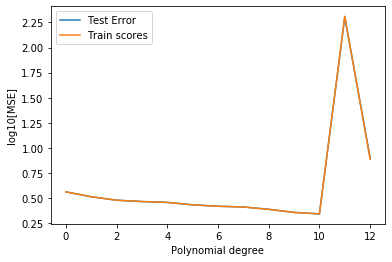
\includegraphics[width=.95\linewidth]{t5}
        \caption{Our code for OLS}
        \label{fig:t3sub1}
    \end{subfigure}%
    \begin{subfigure}{.5\textwidth}
        \centering
        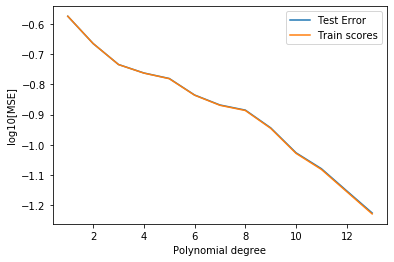
\includegraphics[width=.95\linewidth]{t6}
        \caption{sklearn for OLS}
        \label{fig:t3sub2}
    \end{subfigure}
    \caption{OLS for MSE depending on model complexity}
    \label{fig:t3}
\end{figure}

We suspect this may be due to numerical instability that since we are having now higher degree polynomials where small values like 0.1 or 0.01 might be taken to the 11th or 12th power which leads to values very close to zero which our matrix inversion can't handle anymore.

When using cross-validation we get very similar pictures.

\subsubsection{Ridge regression}

When using Ridge regression, we try to find the best $\lambda$ to reduce the MSE-score (still using up to degree 5 polynomials). Here it seems like the best lambda is a very small lambda and increasing lambda will only make the MSE worse, see figure \ref{fig:t4}.

\begin{figure}
    \centering
    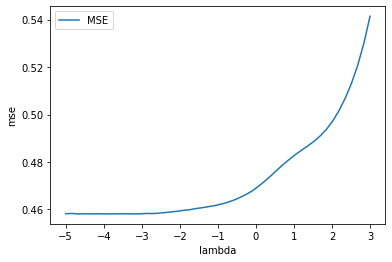
\includegraphics{t7}
    \caption{MSE depending on $\lambda$ for up to degree 5 polynomials for Ridge}
    \label{fig:t4}
\end{figure}

We observe the same thing if we vary the complexity of the model (figure \ref{fig:t5}). For lower degree polynomials the difference is smaller than for higher the degree polynomials but the pattern stays that the higher the $\lambda$ and thus the further away the Ridge fit from the OLS the higher the MSE-score is.

\begin{figure}
    \centering
    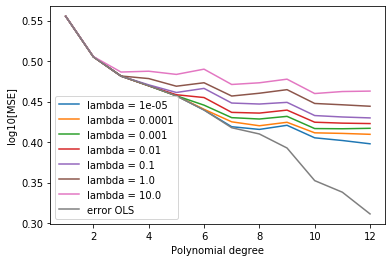
\includegraphics{t8}
    \caption{MSE depending on $\lambda$ and model complexity for Ridge}
    \label{fig:t5}
\end{figure}

\subsubsection{Lasso regression}

\begin{figure}
    \centering
    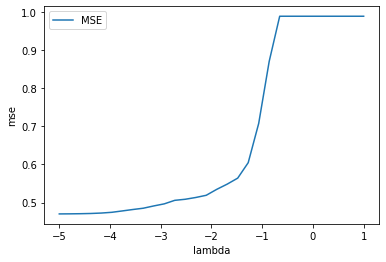
\includegraphics{lasso_lambda}
    \caption{MSE depending on $\lambda$ for up to degree 5 polynomials for Lasso}
    \label{fig:t6}
\end{figure}

Again very similar results in this case. The MSE-score increases the higher the $\lambda$ and the best $\lambda$ should be the lowest one(figure \ref{fig:t6}). At some point it MSE doesn't increase anymore, the reason for this should be that Lasso actually may set coefficients as zero whereas Ridge just makes them smaller by a factor dependent on $\lambda$. And exactly the same applies if you additionally vary the model complexity (figure \ref{fig:t7}). It seems though that Lasso is even a little bit worse than Ridge.

\begin{figure}
    \centering
    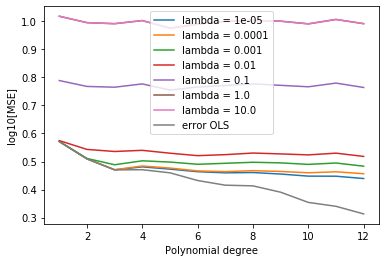
\includegraphics{lasso_lambdas_complexity}
    \caption{MSE depending on $\lambda$ and model complexity for Lasso}
    \label{fig:t7}
\end{figure}

\section{Conclusions}

In this report we started by looking at the Franke function, a continuous, two-dimensional function. We fitted three different regression models to this function; OLS regression, Ridge regression and LASSO regression. Cross-validation was used as resampling technique to properly assess the different models. The three models are compared on their MSE-score and $R^2$-score, both for the training and test data, and in the end also for the real data without the noise. We started by assessing the MSE-score for OLS as a function of the model complexity, where we showed that the optimal polynomial degree, which gives the lowest MSE-score, is a degree of seven. We also assessed the bias-variance tradeoff as a function of the complexity of the model, which confirmed our initial optimal polynomial degree of seven. 

Using this polynomial degree, we looked at the values for $\lambda$ for the Ridge regression. It turned out that the smaller $\lambda$ gets, the lower the MSE-score for Ridge, already indicating that Ridge might not be a better fit. We also discussed the MSE-score and bias-variance tradeoff for different values of $\lambda$ and model complexity. Here we also saw that the smaller $\lambda$, the lower the MSE-score. We found that the optimal value for $\lambda$ is $10^{7}$. We also saw that the MSE-score of OLS was still lower than the MSE-score for Ridge regression. 

Then we looked at LASSO regression, where we also found that the smaller the value for $\lambda$, the lower the MSE-score. We found that the optimal value for $\lambda$ is $10^{7}$. 

When comparing the MSE-scores and $R^2$-scores for the three different models, with their optimal hyperparameters, we saw that for the Franke function, the OLS regression gave the best scores. However, Ridge regression gave almost the same results.

The observation sort of, although we are not sure to what extent there is a causal relation, aligns with the conceptual reasoning that if you just want to approximate an exponential function(or a sum of these) we remember that in the taylor series expansion of an exponential function no coefficient in front of the polynomials is zero. So when fitting with these models you are kind of trying to figure out which coefficients should be in front of each of those polynomials(?). However, by penalizing the size of the entries of beta some of these coefficients get set to zero by the Lasso regression which basically doesn't really fit to the fact that the coefficients in the the taylor series are not. This may explain why especially Lasso is not as good as OLS.

For the real data it seems like there is no benefit at all to Ridge or Lasso. This also might be due to since we are using a lot of data points, so it is hard to overfit. If we would use less data overfitting probably would occur and the decrease in variance due to Ridge and Lasso would start to make a difference.


Again very, very sketchy and not sure if this makes sense at all!(similar arguments to above):
If we assume, we can model our terrain data by an analytic function (meaning we have a convergent power series) very well and since we have real data the coefficients are "basically random" they are very likely not going to be zero and the term they are standing in front of makes a contribution which is not the case when Lasso shrinks some coefficients to be actually zero.

\section{Appendix}

\subsection{Model complexity}

\begin{figure}
    \centering
    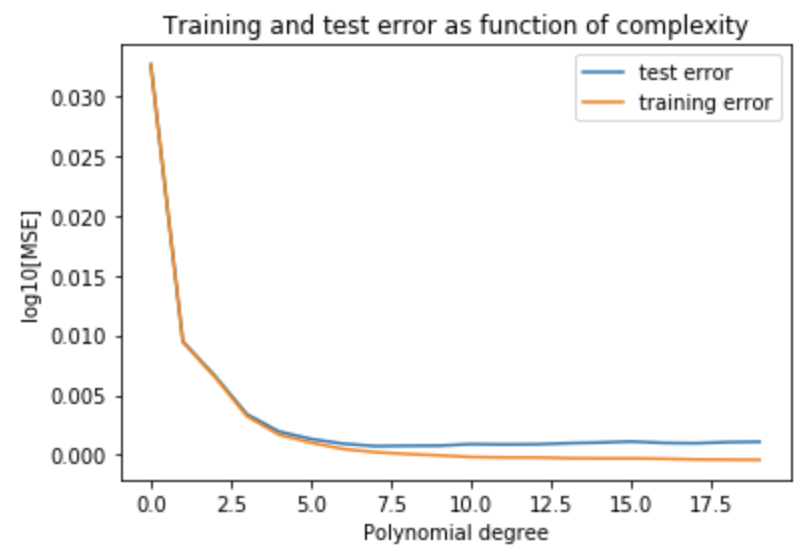
\includegraphics[width=0.9\linewidth]{13}
    \caption{Comparing training and test error}
    \label{fig:f11}
\end{figure}

In figure \ref{fig:f11} we see that for a polynomial degree in the order of zero and one the error is relatively so big that the rest of the graph is not readable anymore.

\begin{figure}
    \centering
    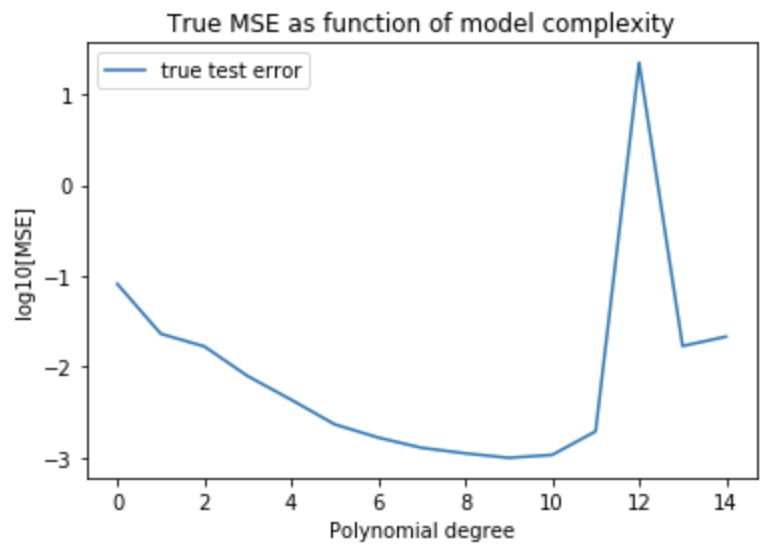
\includegraphics[width=0.9\linewidth]{14}
    \caption{Error on test data}
    \label{fig:f12}
\end{figure}

This graph shows that for a polynomial of 7 we also have a low MSE-score for the real function. However, interpreting the results of this graph should be with caution, since there is no cross-validation used this graph is based on a small sample of the data, and on one run. Even though, it confirms our results. 

\clearpage

\bibliographystyle{plain}
\bibliography{M335}

\end{document}